\documentclass[10pt]{extarticle}

%Paquetes utilizados en esta tarea
\usepackage{fullpage}
\usepackage[utf8]{inputenc}
\usepackage[spanish]{babel}
\usepackage{epsfig}
\usepackage{amsmath}
\usepackage{amssymb}
\usepackage{epstopdf}
\usepackage[hidelinks]{hyperref}
\usepackage{xcolor}
\usepackage{algorithmic}
\usepackage[nothing]{algorithm}

%Definiciones de comandos, para reutilizar secuencias frecuentes o ahorrar
%código
\newcommand{\RR}{\mathbb{R}}
\newcommand{\lb}{\\~\\}
\newcommand{\la}{\leftarrow}

\newcommand{\twopartdef}[4]
{
	\left\{
		\begin{array}{ll}
			#1 &  \text{si }#2 \\
			#3 &  \text{si }#4
		\end{array}
	\right.
}

\newcommand{\threepartdef}[6]
{
	\left\{
		\begin{array}{ll}
			#1 &  \text{si }#2 \\
			#3 &  \text{si }#4 \\
			#5 &  \text{si }#6
		\end{array}
	\right.
}

\makeatletter

\makeatother

\begin{document}

\begin{tabular}{ccl}
 \begin{tabular}{c}
 
\includegraphics[width=2.5cm]{imgs/logo.pdf}
\end{tabular}
&\ \ \ &
\begin{tabular}{l}
 PONTIFICIA UNIVERSIDAD CATÓLICA DE CHILE               \\
 DEPARTAMENTO DE CIENCIA DE LA COMPUTACIÓN              \\
 IIC3524 {-} Tópicos avanzados de sistemas distribuidos \\
\end{tabular}
\end{tabular}

\begin{center}
 \bf {\Huge Tarea 2}

 \vspace{0.2cm}
 \bf 27 de junio de 2017

 \vspace{0.2cm}
 \bf Nicolás Gebauer {-} 13634941

 \vspace{0.2cm}
 \bf \href{https://github.com/negebauer}{\color{blue!60} @negebauer} {-} \href{https://github.com/negebauer/IIC3524-T2}{\color{blue!60}repo T2}
 \noindent\rule{16cm}{0.05pt}

 \vspace{0.5cm}
 % \bf {\huge Análisis}
\end{center}

\subsection*{Análisis de rendimiento}
Se ejecutó el programa en su versión secuencial y paralela. La versión paralela se corrió con 4 procesos en cada nodo. Los nodos utilizados fueron 3, tripio, trauco y caleuche.\\
Los tiempos de procesamiento para encontrar el camino más corto, junto con los speedups respectivos, se presentan a continuación.\\
Las tablas describen para cada test el tiempo que tomo ejecutando \textit{time} en los campos \textit{real} y \textit{user}. S son los tiempos secuenciales, P los paralelos.

\begin{center}
 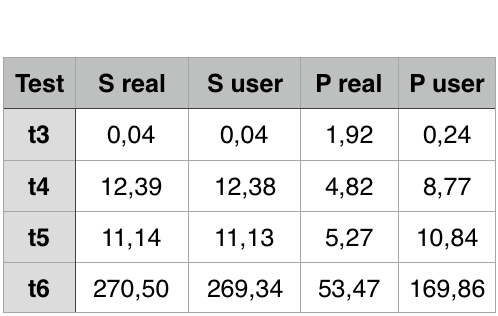
\includegraphics[width=6cm]{imgs/table_seconds.png}\\
 \footnotesize{Tiempos de ejecución en segundos}\\
\end{center}

\begin{center}
 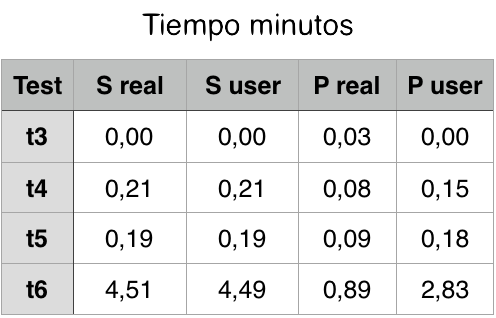
\includegraphics[width=6cm]{imgs/table_minutes.png}\\
 \footnotesize{Tiempos de ejecución en minutos}\\
\end{center}

\begin{center}
 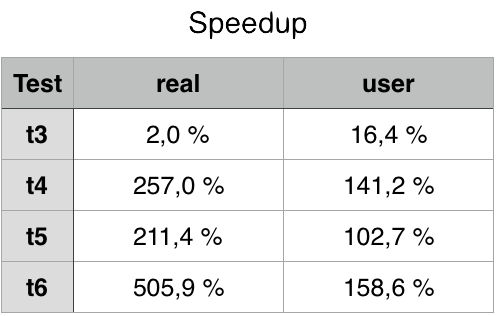
\includegraphics[width=6cm]{imgs/table_speedup.png}\\
 \footnotesize{Speedups}\\
\end{center}

Se grafican las tablas de tiempo y speedup a continuación

\begin{center}
 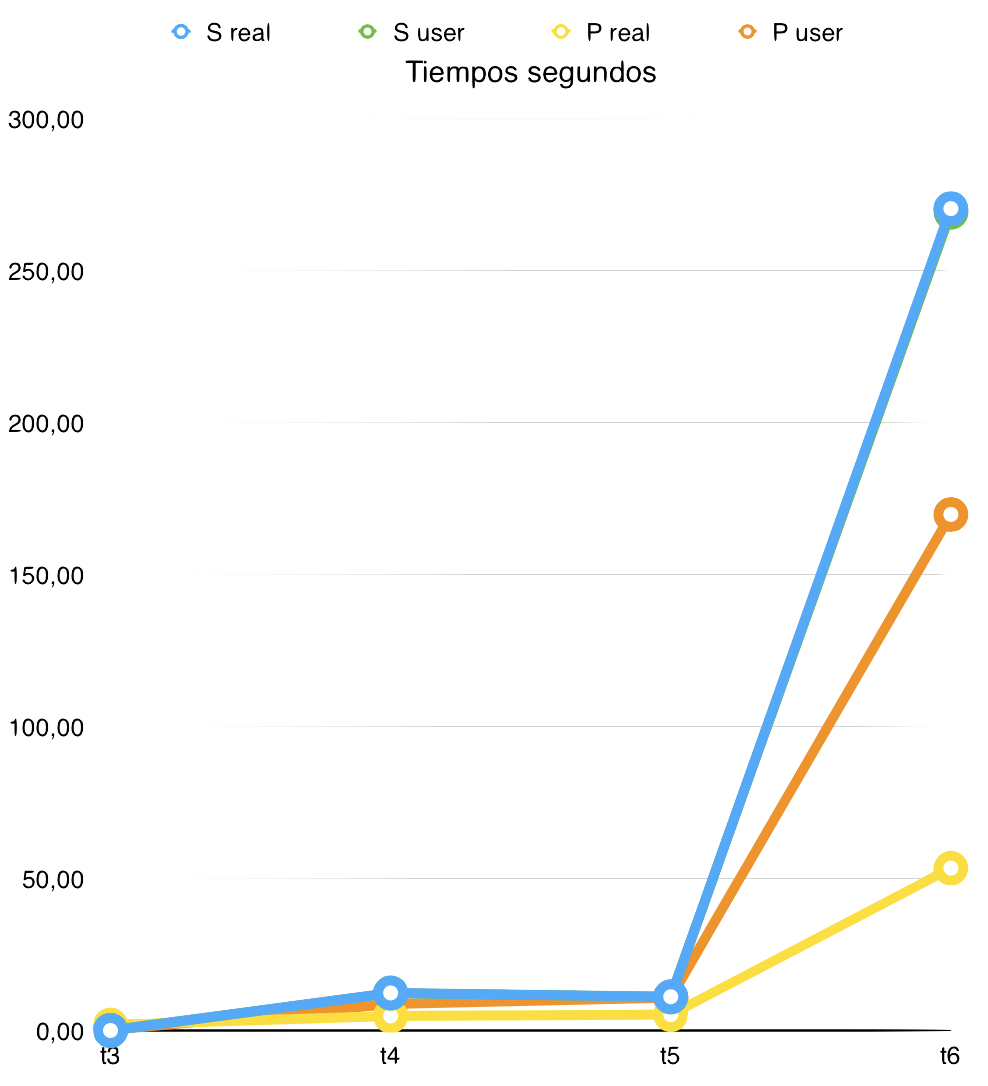
\includegraphics[width=6cm]{imgs/graph_seconds.png}\\
 \footnotesize{Tiempos de ejecución en segundos}\\
\end{center}

\begin{center}
 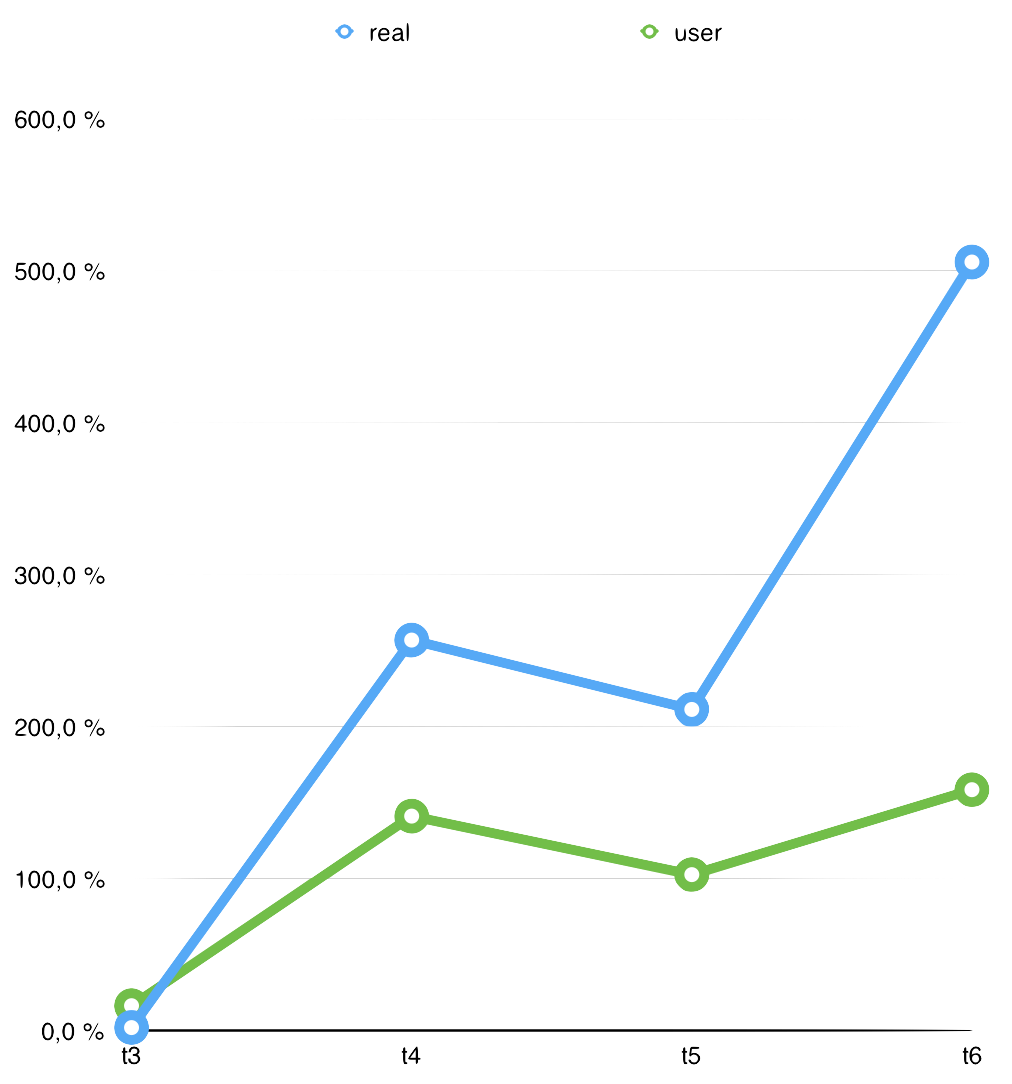
\includegraphics[width=6cm]{imgs/graph_speedup.png}\\
 \footnotesize{Speedups}\\
\end{center}


\textit{./run.sh test/img/big.png test/kernel/blur\_3.txt 3}\\

Antecedido por \textit{OMP\_NUM\_THREADS=n} con $n$ de 1 a 16.\\

\begin{center}
 \includegraphics[width=12cm]{imgs/big_threads.png}\\
 \footnotesize{Tiempos CPU con 1 a 16 threads. Comando usado:}\\
\end{center}


\begin{center}
 \includegraphics[width=12cm]{imgs/big_threads_speedup.png}\\
 \footnotesize{Speedup con 1 a 16 threads. Comando usado:}\\
\end{center}

\subsection*{Discusión}
Debe efectuar un ana ́lisis comparando el tiempo de ejecucio ́n, speedup y eficiencia para diferentes valores de N y cantidad de procesos MPI, y reportar gra ́ficamente estos valores. Utilice valores de N representativos que permitan apreciar una diferencia en tiempo de ejecucio ́n.
Para efectos de comparacio ́n, la versio ́n baseline debe ser la versio ́n MPI ejecutado usando solamente un proceso local.
Debe escribir un informe donde describa sus experimentos y discuta los resultados.

Se aprecia que al aumentar el número de threads disminuye el tiempo que ocupa la CPU cada thread, esto es esperable ya que al dividir la tarea en más procesos cada proceso tendrá que trabajar menos. También el tiempo total de uso de la CPU aumenta al aumentar el número de threads. Esto también es esperable ya que al tener más procesos que corren sobre la CPU es uso total es mayor. Es importante destacar que este tiempo no es cuanto demora el programa, sino más bien cuanto tiempo de cómputo usa de la CPU (en su totalidad). A partir de los 8 threads este valor se estabiliza. Esto puede deberse a que a partir de los 8 threads la CPU se utiliza por completo. Por lo tanto, el tiempo total de uso ya no se puede disminuir. Tener más threads solo hace que cada thread trabaje menos, pero el uso total de la CPU se mantiene.\\

Lo importante es el speedup, el cual tiene a disminuir al aumentar la cantidad de threads. Se observa que al pasar de 2 a 3 y de 4 a 5 el speedup disminuye. Esto puede deberse a que el paralelismo funciona mejor con potencias de 2.\\

\end{document}
